\documentclass[11pt]{article}

\def\chapitre{14}
\def\pagetitle{Suites réelles : la théorie.}

\input{/home/theo/MP2I/setup.tex}

\begin{document}

\input{/home/theo/MP2I/title.tex}

\thispagestyle{fancy}

\setcounter{section}{-1}

\section{Propriété de la borne supérieure.}

\begin{defi}{}{}
    Soit $A$ une partie de $\R$.
    \begin{itemize}
        \item On appelle \bf{borne supérieure} de $A$ et on note $\sup A$, le plus petit des majorants de $A$, lorsqu'il existe.
        \item On appelle \bf{borne inférieure} de $A$ et on note $\inf A$, le plus grand des minorants de $A$, lorsqu'il existe.
    \end{itemize}
\end{defi}

\quad Implicite dans cette définition : l'unicité de la borne supérieure. On peut la montrer comme on avait prouvé celle du maximum. Pour ce qui concerne l'existence, commençons par examiner un cas simple.

\begin{prop}{}{}
    Si une partie de $\R$ possède un maximum $M$, alors elle a une borne supérieure, qui vaut $M$.
    \tcblower
    Soit $A\subset\R$ admettant un maximum $M$. Soit $M'$ un majorant de $A$, alors $M'\geq M$.\\
    Ainsi, $M$ est le plus petit des majorants : $\sup A = M$.
\end{prop}

\begin{thm}{Axiome de la borne supérieure.}{}
    Toute partie de $\R$ non-vide et majorée admet une borne supérieure dans $\R$.\\
    Toute partie de $\R$ non-vide et minorée admet une borne inférieure dans $\R$.
\end{thm}

\begin{prop}{Caractérisation de la borne supérieure. $\star$}{}
    Soit $A$ une partie de $\R$ non vide et majorée, et $\a\in\R$. On a l'équivalence
    \begin{equation*}
        \a = \sup A \iff \begin{cases}
            \a \nt{ est un majorant de } A\\
            \forall \e > 0, ~ \exists x \in A \mid \a - \e < x \leq \a
        \end{cases}
    \end{equation*}
    \tcblower
    \boxed{\ra} Supposons $\a=\sup A$, c'est un majorant de $A$. Soit $\e>0$. Supposons que $A\cap]\a-\e,\a]=\0$.\\
    Alors $A\subset ]-\infty,\a-\e]$ car $\a$ est majorant de $A$, donc $\a-\e$ majore $A$.\\
    C'est absurde car $\a$ est le plus petit des majorants.\n
    \boxed{\la} Supposons que $\a$ majore $A$ et que $\forall \e > 0, ~ \exists x \in A \mid \a - \e < x \leq \a$.\\
    Supposons qu'il existe $\b<\a$, majorant de $A$. Posons $\e = \a - \b > 0$.\\
    Alors $\b = \a - \e$ : $\exists x \in  A \mid \b < x \leq \a$, absurde car $\b$ majore $A$ : $\a$ est le plus petit des majorants de $A$.
\end{prop}

\begin{ex}{$\star$}{}
    Soit $A=[0,1[$. Justifier l'existence de $\sup A$ puis la calculer.\\
    Soit $B=\{r\in\Q \mid r<\sqrt{2}\}$. Justifier l'existence de $\sup B$ puis la calculer.\\
    Soit $C=\{\frac{1}{n} - \frac{1}{p} \mid (n,p)\in\N^*\}$. Calculer $\sup C$ et $\inf C$, après avoir justifié qu'elles existent.
    \tcblower
    $\bullet~A$ est non vide et majorée par $1$, $\sup A=1$.\\
    $\bullet~B$ est non vide et majorée par $\sqrt{2}$. $\sup B = \sqrt{2}$ par densité de $\Q$ dans $\R$.\\
    $\bullet~C$ est non vide et majorée par $1$, $\sup C=1$, $\inf C = 0$.
\end{ex}

\begin{meth}{Majorer une borne supérieure / passage au sup.}{}
    Soient $M$ un réel et $A$ une partie de $\R$ possédant une borne supérieure. Pour démontrer l'inégalité
    \begin{equation*}
        \sup A \leq M,
    \end{equation*}
    il suffira de montrer que $M$ est un majorant de $A$.
\end{meth}

\begin{ex}{$\star$}{}
    Soient $A$ et $B$ deux parties non-vides et majorées de $\R$ telles que $A\subset B$.\\
    Justifier que $\sup A \leq \sup B$.
    \tcblower
    Puisque $A\subset B$, on a $\sup B$ majorant de $A$, or $\sup A$ est le plus petit des majorants de $A$, donc $\sup A \leq \sup B$. 
\end{ex}

\begin{ex}{Homogénéité du sup. $\star$}{}
    Soit $A$ une partie de $\R$ non vide et majorée et $\l\in\R_+^*$. On définit la partie $\l A := \{\l x \mid x \in A\}$.\\
    Montrer l'égalité
    \begin{equation*}
        \sup(\l A) = \l\sup(A).
    \end{equation*}
    \tcblower
    Soit $x\in A$.\\
    \boxed{\leq} On a $x\leq\sup(A)$ donc $\l x \leq \l \sup(A)$ donc $\l\sup(A)$ majore $\l A$ : $\l\sup(A)\geq\sup(\l A)$.\\[0.1cm]
    \boxed{\geq} On a $\l x \leq \sup(\l A)$ donc $x\leq \frac{1}{\l}\sup(\l A)$ donc $\sup(A)\leq \frac{1}{\l}\sup(\l A)$ donc $\l\sup(A)\leq\sup(\l A)$.\\[0.1cm]
    Par double inégalité, on a $\sup(\l A) = \l\sup(A)$. 
\end{ex}

\section{Limite d'une suite.}

\begin{defi}{Convergence vers $l\in\R$}{}
    Soit $(u_n)_{n\in\N}$ une suite réelle et $l\in\R$. On dit que $(u_n)$ \bf{converge} vers $l$ et on note $u_n\to l$ si
    \begin{equation*}
        \forall \e > 0, ~ \exists n_0 \in \N ~ \mid ~ \forall n \geq n_0 ~ : ~ |u_n - l| \leq \e
    \end{equation*}
\end{defi}

\quad Cette définition est écrite sous cette forme par Cauchy en 1821. Elle avait été donnée par d'Alembert dans l'Encyclopédie (1767) : \emph{<< On dit qu'une grandeur est la limite d'une autre grandeur quand la seconde peut approcher la première plus près que d'une grandeur donnée si petite qu'on la puisse supposer... >>}

\begin{prop}{}{}
    Soit $(u_n)_{n\in\N}$ et $l\in\R$. On a
    \begin{equation*}
        u_n \to l \iff |u_n - l| \to 0
    \end{equation*}
    \tcblower
    Par équivalences :
    \begin{align*}
        u_n \to l &\iff \forall \e > 0, ~ \exists n_0 \in \N \mid \forall n \geq n_0 ~ : ~ |u_n - l| \leq \e \\&\iff \forall \e > 0, ~ \exists n_0 \in \N \mid \forall n \geq n_0 ~ : ~ ||u_n - l| - 0| \leq \e \\&\iff |u_n - l| \to 0
    \end{align*}
\end{prop}

\begin{meth}{}{}
    Prouver une convergence du type $u_n\to l$, c'est montrer que la \bf{distance} $|u_n-l|$ peut être rendu << aussi petite que l'on veut >>. On cherchera donc
    \begin{itemize}
        \item À majorer $|u_n - l|$ par un réel $\e$ quelconque à partir d'un certain rang $n_0$ qui dépend de $\e$. C'est ce que nous ferons dans les preuves de ce cours mais dans les exercices, on dégainera rarement $\e$ !
        \item À majorer $|u_n - l|$ par une suite convergeant notoirement vers 0. On peut alors conclure grâce au théorème d'encadrement.
    \end{itemize}
\end{meth}

\begin{ex}{}{}
    \begin{itemize}
        \item Soit $(u_n)$ une suite constante égale à $a\in\R$. Démontrer que $u_n\to a$.
        \item Soit la suite $(u_n)$ de terme général $u_n=\frac{n+1}{n}$.\\
        Démontrer que $u_n\to l$ où $l$ est un réel à déterminer.
    \end{itemize}
    \tcblower
    $\boxed{1.}$ Soient $\e>0$, $\forall n \geq 0, ~ |u_n - a| = |a - a| = 0 \leq \e$ donc $u_n\to a$.\\
    $\boxed{2.}$ Soit $\e>0$. On pose $n_0=\lc\frac{1}{\e}\rc$. Alors $\forall n \geq n_0, ~ |u_n - 1| = \frac{1}{n}\leq\frac{1}{n_0}\leq\e$ par décroissance de $(u_n)$.\\
    Donc $u_n\to 1$. 
\end{ex}

\begin{defi}{}{}
    Soit $(u_n)$ une suite réelle. On dit qu'elle \bf{tend vers} $+\infty$ et on note $u_n\to+\infty$ si
    \begin{equation*}
        \forall M > 0, ~ \exists n_0 \in \N ~ \mid ~ \forall n \geq n_0 ~ : ~ u_n \geq M.
    \end{equation*}
\end{defi}

\begin{ex}{}{}
    Pour $n\geq2$, posons $u_n=\ln(\ln(n))$. Montrer que $u_n\to+\infty$.
    \tcblower
    Soit $M>0$. On pose $n_0=\exp(\exp(M))$, alors $u_{n_0}=M$ et $\forall n\geq n_0, ~ u_n \geq u_{n_0} = M$ car $\ln$ est croissante.\\
    Donc $u_n\to+\infty$.
\end{ex}

\begin{prop}{Tendre vers $-\infty$}{}
    Soit $(u_n)$ une suite réelle. On dit qu'elle \bf{tend} vers $-\infty$ et on note $u_n\to-\infty$ si
    \begin{equation*}
        \forall M < 0, ~ \exists n_0 \in \N ~ \mid ~ \forall n \geq n_0 ~ : ~ u_n \leq M.
    \end{equation*}
    On a l'équivalence $u_n\to-\infty \iff -u_n \to +\infty$.
    \tcblower
    Par équivalences :
    \begin{align*}
        u_n \to -\infty &\iff \forall M < 0, ~ \exists n_0 \in \N ~ \mid ~ \forall n \geq n_0 ~ : ~ u_n \leq M\\
        &\iff \forall M < 0, ~ \exists n_0 \in \N ~ \mid ~ \forall n \geq n_0 ~ : ~ -u_n \geq  -M\\
        &\iff \forall M > 0, ~ \exists n_0 \in \N ~ \mid ~ \forall n \geq n_0 ~ : ~ -u_n \geq M\\
        &\iff -u_n \to +\infty
    \end{align*}
\end{prop}

\begin{prop}{Unicité de la limite.}{}
    Soit $(u_n)$ une suite réelle et $L,L'\in\ov{R}$. Si $u_n\to L$ et $u_n\to L'$, alors $L=L'$.\\
    Le nombre $L$ est alors appelé limite de la suite $(u_n)$ et noté $\lim u_n$.
    \tcblower
    Dans le cas où les deux limites sont finies...\\
    Soit $\e>0$, $\exists n_1 \in \N \mid \forall n \geq n_1, ~ |u_n - L| \leq \e$ et $\exists n_2 \in \N \mid \forall n \geq n_2, ~ |u_n - L'| \leq \e$.\\
    Posons $n_0 = \max(n_1,n_2)$, et $n\geq n_0$. Alors $|u_n-L|\leq \e$ et $|u_n-L'|\leq\e$.
    \begin{equation*}
        |L-L'| = |L - u_n + u_n - L'| \leq |L - u_n| + |u_n - L'| \leq 2\e.
    \end{equation*}
    Donc $|L-L'|\leq 2\e$ pour tout $\e>0$, donc $L=L'$.
\end{prop}

\begin{defi}{}{}
    On dit d'une suite $(u_n)$ qu'elle est \bf{convergente} si elle converge vers une limite finie. Si une suite n'est pas convergente, elle est dite \bf{divergente}.
\end{defi}

\begin{ex}{}{}
    On démontre que la suite de terme général $(-1)^n$ est divergente.
    \tcblower
    Supposons qu'il existe $l\in\R$ tel que $(-1)^n\to l$. Posons $\e=\frac{1}{2}$, $\exists n_0\in\N\mid\forall n\geq n_0, ~ |u_n-l|\leq \frac{1}{2}$. Soit $n\geq n_0$.\\
    D'une part, $|u_{n+1}-l+l-u_n|\leq|u_{n+1}-l|+|u_n-l|=\frac{1}{2}+\frac{1}{2}=1$.\\
    D'autre part, $\forall n \in \N, ~ |u_{n+1} - u_n| = 2$.
    Alors $2 \leq 1$, absurde. Donc $(-1)^n$ est divergente.
\end{ex}

\begin{prop}{}{}
    Toute suite convergente est bornée.
    \tcblower
    Soit $(u_n)$ convergente de limite $l$. Soit $\e=1$, $\exists n_0\in\N\mid\forall n\geq n_0, ~ |u_n-l|\leq 1$.\\
    Posons $T_{n_0}=\{u_k \mid k\in\lb0,n_0\rb\}$. C'est un ensemble fini, de cardinal inférieur à $n_0$. Ainsi, il possède un maximum et un minimum, qu'on note $M$ et $m$.
    Alors $\forall n \in \N, ~ u_n \in [\min(m,l-1), \max(M,l+1)]$, elle est bornée.
\end{prop}

La réciproque est fausse : la suite de terme général $(-1)^n$ est bornée et divergente.

\pagebreak

\section{Limites et opérations : preuves des résultats.}

\quad On démontre ici une partie seulement de tous les résultats ayant été donnés sous forme de tableaux dans le cours Suites réelles : la pratique.

\begin{prop}{Somme de deux suites ayant une limite. $\star$}{}
    Soient $(u_n)$ et $(v_n)$ deux suites réelles, et $l,l'$ deux nombres réels.
    \begin{center}
        Si $u_n\to l$ et $v_n\to l'$, alors $u_n + v_n\to l + l'$.\\
        Si $u_n\to l$ et $v_n \to +\infty$, alors $u_n+v_n\to+\infty$.
    \end{center}
    \tcblower
    $\star$ Supposons que $u_n\to l$ et $v_n\to l'$. Soit $\e>0$.\\
    On a $\exists n_1 \in \N \mid \forall n \geq n_1, ~ |u_n - l| \leq \frac{\e}{2}$ et $\exists n_2 \in \N \mid \forall n \geq n_2, ~ |v_n - l'| \leq \frac{\e}{2}$.\\
    On pose $n_0=\max(n_1,n_2)$. Pour $n\geq n_0$, on a :
    \begin{equation*}
        |(u_n + v_n) - (l + l')| = |(u_n - l) + (v_n - l')| \leq |u_n - l| + |v_n - l'| \leq \frac{\e}{2} + \frac{\e}{2} = \e
    \end{equation*}
    On a bien $u_n + v_n \to l + l'$.\n
    $\bullet$ Supposons que $u_n \to l$ et $v_n \to +\infty$. Soit $M>0$.\\
    On a $\exists n_1 \in \N \mid \forall n \geq n_1, ~ u_n\in[l-1, l+1]$ et $\exists n_2\in\N\mid \forall n \geq n_2, ~ v_n \geq M - (l - 1)$.\\
    Pour $n\geq\max(n_1,n_2)$, on a $u_n+v_n\geq l-1 + M - (l-1) = M$, donc $u_n+v_n\to+\infty$.
\end{prop}

\begin{lemme}{}{}
    Le produit d'une suite bornée et d'une suite de limite nulle est une suite de limite nulle.
    \tcblower
    Soient $u$ et $v$ deux suites réelles telles que $u_n\to 0$ et $v$ bornée. Soit $\e>0$.\\
    Puisque $v$ est bornée, $(|v_n|)$ est majorée : $\exists M > 0 \mid \forall n \in \N, ~ |v_n| \leq M$.\\
    Puisque $u_n\to0$, $\exists n_0\in\N \mid \forall n \geq n_0, ~ |u_n-0|\leq\frac{\e}{M}$.\\
    Alors : $\forall n \geq n_0, ~ |u_nv_n|=|u_n||v_n|\leq \frac{\e}{M}M=\e$
\end{lemme}

\begin{lemme}{}{}
    Si $(u_n)$ converge vers $l>0$, alors $u_n>\frac{l}{2}$ à partir d'un certain rang, en particulier $u_n>0$ à.p.d.c.r.
    \tcblower
    Prenons $\e=\frac{l}{2}$. On a $\exists n_0 \in \N \mid \forall n\geq n_0, ~ u_n \in [l-\frac{l}{2},l+\frac{l}{2}]$. En particulier, $\forall n \geq n_0, ~ u_n \geq \frac{l}{2} > 0$.
\end{lemme}

\begin{prop}{Produit de deux suites ayant une limite. $\star$}{}
    Soient $(u_n)$ et $(v_n)$ deux suites réelles, et $l,l'$ deux nombres réels.
    \begin{center}
        Si $u_n\to l$ et $v_n\to l'$, alors $u_nv_n\to ll'$.\\
        Supposons $l>0$. Si $u_n\to l$ et $v_n\to+\infty$, alors $u_nv_n\to+\infty$.
    \end{center}
    \tcblower
    $\star$ Supposons $u_n\to l$ et $v_n\to l'$.\\
    Soit $\e>0$ : $\exists n_1 \in \N \mid \forall n \geq n_1, ~ |u_n||v_n - l'| \leq \e$ et $\exists n_2 \in \N \mid \forall n \geq n_2, ~ |l'||u_n - l| \leq \e$.\\
    Pour $n\geq\max(n_1,n_2)$, on a:
    \begin{align*}
        |u_nv_n-ll'| &= |u_n(v_n-l') + u_nl' -ll'| = |u_n(v_n-l') + l'(u_n-l)|\\
        &=|u_n||v_n-l'| + |l'||u_n-l|\leq 2\e
    \end{align*}
    Donc $u_nv_n\to ll'$.\n
    $\bullet$ Supposons $u_n\to l>0$ et $v_n\to+\infty$. Soit $M>0$ : $\exists n_0'\in\N \mid \forall n \geq n_0' ~ v_n\geq\frac{2M}{l}$.\\
    D'après le lemme, on a : $\exists n_0 \in \N \mid \forall n \geq n_0, ~ u_n\geq\frac{l}{2}$. Donc pour $n\geq\max(n_0,n_0')$ : $u_nv_n\geq\frac{l}{2}\cdot\frac{2M}{l}\geq M$.
\end{prop}

\begin{prop}{Inverse, quotient de deux suites ayant une limite.}{}
    Soient $(u_n)$ et $(v_n)$ deux suites réelles, et $l,l'$ deux nombres réels, avec $l\neq0$.
    \begin{center}
        Si $(u_n)\to0_+$, alors $\ds\frac{1}{u_n}\to+\infty$. \qquad Si $u_n\to l$ et $v_n\to l'$, alors $\ds\frac{u_n}{v_n}\to\frac{l}{l'}$. 
    \end{center}
    \tcblower
    $\bullet$ Supposons $u_n\to0_+$. Soit $M>0$, on pose $\e=M^{-1}$.\\
    Puisque $u_n\to0_+$, on a $0\leq u_n \leq M^{-1}$ àpdcr, donc $u_n^{-1}\geq M$ àpdcr.
\end{prop}

\begin{prop}{Lemme de Cesàro.}{}
    Soit $(u_n)_{n\geq1}$ une suite réelle et $l\in\R$.\\
    Pour $n\in\N^*$, on note $c_n$ la moyenne arithmétique des $n$ premiers termes de $\ds u: c_n = \frac{1}{n}\sum_{k=1}^nu_k$.\\
    Si $u_n\to l$, alors $c_n\to l$.
\end{prop}

\section{Passer à la limite ?}

Les propositions ci-dessous examinent la possibilité de passer à la limite dans une inégalité ou une égalité.

\begin{prop}{Passage à la limite d'une inégalité large.}{}
    Soient $u$ et $v$ deux suites réelles et $l$, $l'$ deux réels.
    \begin{equation*}
        \nt{Si} ~ \begin{cases}\forall n \in \N, ~ u_n \leq v_n \\ u_n \to l ~\et~ v_n \to l'\end{cases} \quad \nt{alors} ~ l \leq l'.
    \end{equation*}
    En particulier,
    \begin{itemize}
        \item si $u$ est majorée par $M\in\R$ et admet une limite, alors $\lim u_n \leq M$.
        \item si $u$ est minorée par $m\in\R$ et admet une limite, alors $\lim u_n \geq m$.
    \end{itemize}
    \tcblower
    \bf{Cas particulier.} Supposons que $\forall n\in\N, ~ u_n \leq M$ et $u_n \to l$. Par l'absurde, supposons $l\> M$.\\
    On pose $\e=\frac{l-M}{2}>0$. Puisque $u_n\to l$, $\exists n_0 \in \N, ~ u_{n_0} \in [l-\e, l + \e]$, absurde car alors $u_{n_0} > M$.\\
    Donc $l\leq M$. Même preuve pour le cas minoré.\n
    \bf{Cas général.} Supposons que $\forall n \in \N, ~ u_n \leq v_n$, que $u_n \to l$ et que $v_n \to l'$.\\
    On a $(v_n - u_n)$ minorée par $0$ et $v_n-u_n \to l' - l$.\\
    D'après le cas particulier, $l'-l \geq 0$ donc $l\leq l'$.
\end{prop}

\warning Les inégalités structes ne sont \bf{pas} conservées : $\forall n \in \N^*, ~ \frac{1}{n}>0$ et $\lim\frac{1}{n}=0$.

\begin{ex}{}{}
    Soit $(u_n)$ la suite définie par : $\ds\begin{cases}u_0 \in \R\\ \forall n \in \N, ~ u_{n+1} = u_n - u_n^2\end{cases}$
    \begin{enumerate}
        \item Que dire de la monotonie de $u$ ?
        \item Supposons $u_0\in[0,1]$. Montrer que $(u_n)$ est convergente et que $\lim u_n = 0$.
        \item Supposons que $u_0 < 0$. Montrer que $(u_n)\to-\infty$. Que dire si $u_0>1$ ?
    \end{enumerate}
    \tcblower
    \boxed{1.} Soit $n\in\N$. $u_{n+1}-u_n=-u_n^2\leq0$ donc $(u_n)$ est décroissante.\\
    \boxed{2.} Supposons $u_0\in[0,1]$, Par récurrence, on montre que $u_n\geq0$. Vrai pour $u_0$.\\
    Soit $n\in\N$ tel que $u_n\geq0$, alors $u_{n+1}=u_n(1-u_n)\geq0$ donc $u$ est minorée par 0 par récurrence.\\
    La suite est décroissante et minorée donc elle converge par TLM, on note $l$ sa limite.\\
    On a $l=l-l^2$ par passage à la limite donc $l=0$.\\
    \boxed{3.} Supposons $u_0<0$ et $u$ minorée. Par TLM, $u$ converge, on note $l$ sa limite, alors $l=0$.\\
    Par décroissance de $u$, $\forall n \in \N, ~ u_n \leq u_0$ donc $l \leq u_0$ donc $0 \leq u_0 < 0$, absurde.\\
    Donc $u$ n'est pas minorée : elle diverge vers $-\infty$. Quand $u_0>1$, $u_1 < 0$.
\end{ex}

\quad Voici un résultat utilisé pour obtenir une équation sur la limite d'une suite convergente définie par une relation du type << $u_{n+1}=f(u_n)$ >>.

\begin{prop}{La limite comme point fixe.}{}
    Soit $X\in\P(\R)$, $f:X\to X$ et $u$ une suite satisfait $u_0\in X$ et $\forall n \in \N, ~ u_{n+1}=f(u_n)$.\\
    Si $(u_n)$ converge vers une limite $l$, que $l\in I$ et que $f$ est continue en $l$, alors $f(l)=l$.
    \tcblower
    On a $u_{n+1}=f(l)$ et $u_{n+1}\to l$ donc $u_n\to l$ donc $f(u_n)\to f(l)$ car $f$ est continue en $l$.\\
    Alors $f(l)=l$.
\end{prop}

\begin{ex}{}{}
    Soit $(u_n)$ une suite réelle telle que $\forall n \in \N, ~ u_{n+1} = \ch(u_n)$. Démontrer que $(u_n)$ diverge.
    \tcblower
    Supposons $u$ convergente vers $l\in\R$, alors $l=\ch(l)$, or $\ch$ n'a pas de point fixe dans $\R$, absurde donc $u$ diverge.
\end{ex}

\pagebreak

\section{Existence d'une limite : preuve des théorèmes.}

\quad On se concentre ici sur les preuves de résultats qui ont été abondamment utilisés dans le cours \bf{Suites réelles : la pratique}. On y renvoie le lecteur pour les illustrations, les exemples, les corollaires...\n
\quad On rappelle qu'établir un encadrement ou exploiter une monotonie sont les deux stratégies principales face à un problème de convergence de suites.

\fbox{Encadrement.}

\begin{thm}{d'encadrement, ou des gendarmes. $\star$}{}
    Soient trois suites réelles $(g_n), (u_n), (d_n)$ telles que $\forall n\in\N, ~ g_n \leq u_n \leq d_n$.\\
    Si de surcroît, $(g_n)$ et $(d_n)$ convergent vers la limite $l\in\R$, alors
    \begin{center}
        $(u_n)$ est convergente et $\lim u_n = l$.
    \end{center}
    \tcblower
    Soit $\e>0$, $\exists n_1 \in \N \mid \forall n \geq n_1, ~ |g_n - l| \leq \e$ et $\exists n_2 \in \N \mid \forall n \geq n_2, ~ |d_n - l| \leq \e$.\\
    Alors $\forall n \geq \max(n_1, n_2), ~ l - \e \leq g_n \leq  u_n \leq d_n \leq l + \e$ donc $u_n \to l$.
\end{thm}

\begin{prop}{de minoration, de majoration. $\star$}{}
    Soient $(u_n)$ et $(v_n)$ deux suites réelles.
    \begin{itemize}
        \item Si $\forall n \in \N, ~ u_n \leq v_n$ et $v_n \to +\infty$, alors $v_n \to +\infty$.
        \item Si $\forall n \in \N, ~ u_n \leq v_n$ et $v_n \to -\infty$, alors $u_n \to -\infty$.
    \end{itemize}
    \tcblower
    Supposons $\forall n \in \N, ~ u_n \leq v_n$ et $u_n\to+\infty$. Soit $M>0$, $\exists n_0 \in \N \mid \forall n \geq n_0, ~ u_n \geq M$.\\
    Alors $\forall n \geq n_0, ~ v_n \geq u_n \geq M$
\end{prop}

\fbox{Monotonie.}

\begin{thm}{de la limite monotone. $\star$}{}
    Toute suite croissante et majorée converge vers une limite finie.\\
    Toute suite croissante et non majorée diverge vers $+\infty$
    \tcblower
    Soit $(u_n)$ une suite croissante.\\
    $\bullet$ Supposons $u$ majorée : $\exists M \in \R ~ \forall n \in \N, ~ u_n \leq M$.\\
    Posons $T=\{u_n, ~ n \in \N\}$, non vide et majoré : on note $l=\sup(T)$. Soit $\e>0$.\\
    Par caractérisation : $\exists n_0 \in \N ~ s - \e \leq u_{n_0} \leq l$ et par croissance de $u$ : $\forall n \geq n_0, ~ u_{n_0} \leq u_n$.\\
    Ainsi, $\forall n \geq n_0, ~ l - \e \leq u_{n_0} \leq u_n \leq l$. On a bien $u_n\to l$.\\
    $\bullet$ Supposons que $u$ n'est pas majorée. Soit $M>0$, $\exists n_0 \in \N ~ u_{n_0} > M$.\\
    Par croissance de $u$, $\forall n \geq n_0, ~ u_n \geq u_{n_0} > M$ donc $u_n\to+\infty$. 
\end{thm}

\quad On rappelle que deux suites $(u_n)$ et $(v_n)$ sont \bf{adjacentes} lorsqu'elles sont monotones, de monotonie contraire, et que leur différence tend vers 0.

\begin{thm}{Convergence des suites adjacentes. $\star$}{}
    Deux suites adjacentes convergent vers une même limite finie.\n
    Plus précisément, si $(u_n)$ et $(v_n)$ sont deux suites adjacentes ($u$ croissante et $v$ décroissante), alors elles convergent vers une même limite finie $l\in\R$ telle que $\forall n \in \N, ~ u_n \leq l \leq v_n$.
    \tcblower
    Soient $(u_n)$ et $(v_n)$ deux suites adjacentes. On suppose $u$ croissante, $v$ décroissante et $u_n-v_n\to0$.\\
    $\bullet$ $u$ est croissante, par TLM, elle est convergente ou divergente vers $+\infty$.\\
    --- Supposons que $u\to+\infty$. Pour $n\in\N$, $v_n-u_n\leq v_0 - u_n$ par décroissance de $v$.\\
    \hspace*{0.35cm} Ainsi, puisque $u_n\to+\infty$, $v_0-u_n\to-\infty$ donc $v_n-v_n\to-\infty$, absurde donc $u$ converge.\\
    $\bullet$ $v$ est décroissante, par TLM, elle est convergente ou divergente vers $-\infty$.\\
    --- Pour les mêmes raisons, $v_n$ converge.\\
    Notons $l=\lim u_n$ et $l'=\lim v_n$. On a $v_n-u_n\to0$ et $v_n-u_n\to l-l'$ donc par unicité de la limite, $l=l'$.\\
    On a $l$ plus petit majorant de $u$ et plus grand minorant de $v$ d'où $\forall n \in \N, ~ u_n \leq l \leq v_n$.
\end{thm}

\pagebreak

\section{Suites extraites.}

\begin{defi}{}{}
    Soit $(u_n)$ une suite. Une \bf{suite extraite} de $(u_n)$ est une suite $(v_n)$ dont le terme général est de la forme
    \begin{equation*}
        v_n = u_{\phi(n)}
    \end{equation*}
    où $\phi:\N\to\N$ est une application strictement croissante.
\end{defi}

\bf{Exemple.} Soit $(u_n)$ une suite réelle.
\begin{itemize}
    \item Les suites $(u_{2n})$ et $(u_{2n+1})$ sont des suites extraites de $(u_n)$.
    \item D'autres exemples : $(u_{n+1})$, $(u_{n^2})$, $(u_{2^n})$...
\end{itemize}

\begin{lemme}{}{}
    Si $\phi$ est une application strictement croissante de $\N$ dans $\N$ alors, $\forall n \in \N, ~ \phi(n) \geq n$.
    \tcblower
    Soit $\phi:\N\to\N$ strictement croissante. Pour $n\in\N$, on note $\P_n:$ << $\phi(n)\geq\N$ >>.\\
    \bf{Initialisation.} $\phi(0)\in\N$ donc $\phi(0)\geq0$. $\P(0)$ est vraie.\\
    \bf{Hérédité.} Soit $n\in\N$ tel que $\P(n)$ soit vraie. On a $\phi(n+1)>\phi(n)\geq n$ par stricte croissante de $\phi$.\\
    Ainsi, $\phi(n+1)>n$ donc $\phi(n+1)\geq n+1$ car $\phi(n+1)\in\N$.\\
    Par récurrence, $\forall n \in \N, ~ \phi(n) \geq n$.
\end{lemme}

\begin{prop}{}{}
    Soit $(u_n)$ une suite convergente.\\
    Toute suite extraite de $(u_n)$ converge vers la limite de $(u_n)$.
    \tcblower
    Soit $(u_{\phi(n)})$ une suite extraite de $(u_n)$ avec $\phi:\N\to\N$ strictement croissante.\\
    Soit $\e>0$, $\exists n_0 \in \N \mid \forall n \geq n_0, ~ |u_n - l| \leq \e$.\\
    Pour $n\geq n_0$, $\phi(n)\geq\phi(n_0)\geq n_0$ donc $|u_{\phi(n)} - l| \leq \e$.
\end{prop}

\begin{meth}{Prouver la divergence d'une suite avec deux suites extraites.}{}
    Si une suite a deux suites extraites ne convergeant pas vers la même limite, alors elle diverge.
\end{meth}

\begin{ex}{}{}
    Montrer (à nouveau) que la suite de terme général $(-1)^n$ diverge.
    \tcblower
    On a $(-1)^{2n}\to 1$ et $(-1)^{2n+1}\to-1$, donc deux suites extraites de $((-1)^n)$ n'ont pas la même limite.
\end{ex}

\begin{prop}{}{36}
    Soit $(u_n)_{n\geq0}$ une suite réelle et $l\in\R$.
    \begin{center}
        Si $u_{2n}\to l$ et $u_{2n+1}\to l$, alors $u_n \to l$.
    \end{center}
    \tcblower
    Soit $\e>0$, $\exists n_1 \in \N \mid \forall n \geq n_0, ~ |u_{2n}-l|\leq\e$ et $\exists n_2 \in \N \mid \forall n \geq n_2, ~ |u_{2n+1}-l|\leq\e$.\\
    Soit $n_0=\max(n_1,n_2)$. $\forall k \geq 2n_0, ~ |u_k - l| \leq \e$ donc $u_n\to l$.
\end{prop}

\begin{thm}{de Bolzano-Weierstrass.}{}
    Toute suite bornée possède une suite extraite convergente.
\end{thm}

\section{Traduction séquentielle de certaines propriétés.}

\begin{defi}{}{}
    Soit $X$ une partie de $\R$. On dit que $X$ est \bf{dense} dans $\R$ si elle rencontre tout intervalle ouvert de $\R$. Plus précisément, si
    \begin{equation*}
        \forall a < b \in \R, \quad X\cap~]a,b[\neq\0.
    \end{equation*}
\end{defi}

\bf{Exemple.} Dans le cours Propriétés de $\R$, on a démontré que $\Q$ et $\R\setminus\Q$ sont denses dans $\R$.

\pagebreak

\begin{prop}{Caractérisation séquentielle de la densité.}{}
    Soit $X$ une partie de $\R$. Il y a équivalence entre les assetions
    \begin{enumerate}
        \item $X$ est dense dans $\R$.
        \item Pour tout réel $\a$, il existe une suite d'éléments de $X$ qui tend vers $\a$.
    \end{enumerate}
    \tcblower
    Soit $\a\in\R$. \\
    \boxed{\ra} Supposons $X$ dense dans $\R$. Soit $n\in\N^*$.\\
    Par densité de $X$ dans $\R$, $X\cap]\a-\frac{1}{n}, \a + \frac{1}{n}[\neq\0$. Soit $x_n\in X]\a-\frac{1}{n},\a+\frac{1}{n}[$.\\
    Par construction, $(x_n)\in X^\N$ et $\forall n \in \N, ~ \a - \frac{1}{n} \leq x_n \leq \a + \frac{1}{n}$ et par encadrement, $x_n\to\a$.\\
    \boxed{\la} Supposons que $\forall \a \in \R,~ \exists (x_n)\in X^\N \mid x_n \to \a$.\\
    Soient $a,b\in\R$ tels que $a<b$. On pose $\a=\frac{a+b}{2}\in\R$. Alors $\exists (x_n) \in X^\N \mid x_n \to \a$.\\
    Soit $\e>0$ tel que $\e<\frac{b-a}{2}$ : $\exists n_0 \in \N \mid \forall n \geq n_0, ~ |x_n - \a| \leq \e$ alors $x_{n_0}\in]a,b[\cap X$.\\
    On a bien $]a,b[\cap X\neq\0$ donc $X$ est dense dans $\R$.
\end{prop}

\bf{Corollaire.} Tout réel est la limite d'une suite de rationnels. 

\begin{prop}{}{}
    Si $X$ est une partie de $\R$ non-vide majorée (resp. non majorée), alors il existe une suite d'éléments de $X$ de limite $\sup X$ (resp. $+\infty$)
\end{prop}

\section{Suites complexes.}

\begin{defi}{}{}
    Soit $(u_n)_{n\geq0}\in\C^\N$ et $l\in\C$. On dit que $(u_n)$ \bf{converge} vers $l$ et on note $u_n\to l$ si
    \begin{equation*}
        \forall \e > 0, ~ \exists n_0 \in \N \mid \forall n \geq n_0, ~ |u_n - l| \leq \e.
    \end{equation*}
\end{defi}

\begin{prop}{}{}
    Soit $(u_n)_{n\geq0}\in\C^\N$ et $l\in\C$. On a
    \begin{equation*}
        u_n \to l \iff \begin{cases}
            \Re(u_n) \to \Re(l)\\
            \Im(u_n) \to \Im(l)
        \end{cases}
    \end{equation*}
\end{prop}

Restent vraies avec des suites à valeurs complexes :

\begin{itemize}[label=---]
    \item Les résultats sur la limite d'une somme, d'un produit.
    \item Une limite usuelle : si $z\in\C$ est tel que $|z|<1$, alors $z^n\to0$.
    \item L'idée que pour prouver qu'une suite de nombres complexes tend vers 0, on peut écraser son module par une suite qui tend vers 0.
    \item Toute suite de nombres complexes qui converge vers une limite finie est bornée (c'est-à-dire que la suite des modules est majorée).
    \item Bolzano-Weierstrass : de toute suite de nombres complexes bornée (majorée en valeur absolue), on peut extraire une suite convergente.
\end{itemize}

À oublier en revanche : tous les arguments à base d'encadrement ou de monotonie : on rappelle que dans $\C$, on ne dispose pas d'une relation d'ordre.

\section{Exercices}

\subsection*{Borne supérieure d'une partie de $\R$.}

\begin{exercice}{$\bbw$}{}
    Calculer les bornes supérieures et inférieures des parties, après en avoir prouvé l'existence.
    \begin{equation*}
        A=\left\{ \frac{1}{n}+(-1)^n \mid n \in \N^* \right\}, \quad B = \left\{ \frac{m}{nm+1} \mid m \in \N^*, ~ n\in \N^* \right\}, \quad C =\{x^2+y^2 \mid (x,y)\in\R^2 \et xy=1\}.
    \end{equation*}
    \tcblower
    \fbox{A} $A$ est non-vide, minoré par $-1$ et majoré $2$. On note $u$ la suite de terme général $\frac{1}{n}+(-1)^n$.\\
    On a $(u_{2n})$ et $(u_{2n+1})$ décroissantes. De plus, $u_2>u_1$ donc $\sup A = u_2$ et $\inf A = \min(\lim u_{2n}, \lim u_{2n+1})=-1$.\\
    \fbox{B} $B$ est non-vide, minoré par $0$ et majoré par $1$.\\
    À $n$ fixé, $\ds\frac{m}{nm+1}\xrightarrow[m\to+\infty]{}1$ donc $\sup B = 1$ et à $m$ fixé, $\ds\frac{m}{nm+1}\xrightarrow[n\to+\infty]{}0$ donc $\inf B = 0$.\\
    \fbox{C} Posons $f:x\mapsto x^2 + \frac{1}{x^2}$ dérivable sur $\R^*$ avec $f'(x)=2x-\frac{2}{x^3}$. On a:
    \begin{center}
        \begin{tikzpicture}
            \tkzTabInit[espcl=3]{$x$/0.6,$f'(x)$/0.6,$f$/1.0}{$-\infty$,-1,0,1,$+\infty$}
            \tkzTabLine{,-,,+,d,-,,+,}
            \tkzTabVar{+/$+\infty$, -/$2$, +D+/$+\infty$, -/$2$, +/$+\infty$}
        \end{tikzpicture}
    \end{center}
    Donc $\inf C = 2$ et $\sup C = +\infty$.\\
    On a posé cette fonction $f$ car pour tout $x,y\in\R^*,~xy=1 \iff y = x^{-1}$.
\end{exercice}

\begin{exercice}{$\bbw$}{}
    Soient $A$ et $B$ deux aprties non vides et majorées de $\R$. On note $A+B:=\{x+y\mid (x,y)\in A\times B\}$. Démontrer
    \begin{equation*}
        \sup(A+B)=\sup(A)+\sup(B)
    \end{equation*}
    \tcblower
    \boxed{\leq} Soit $x\in A+B$, $\exists a,b \in A\times B \mid x = a + b$. On a $a\leq\sup(A)$ et $b\leq\sup(B)$ donc $x\leq\sup(A)+\sup(B)$.\\
    On a donc $\sup(A+B)\leq\sup(A)+\sup(B)$.\\
    \boxed{\geq} Soient $a,b\in A\times B$ on a $a+b\leq\sup(A+B)$ donc $a\leq\sup(A+B)-b$ donc $\sup(A)\leq\sup(A+B)-b$.\\
    Ainsi, $b\leq\sup(A+B) - \sup(A)$, d'où $\sup(A)+\sup(B)\leq\sup(A+B)$.
\end{exercice}

\subsection*{Suites convergentes : quelques exercices de plus.}

\begin{exercice}{$\bbw$}{}
    Soit $(u_n)$ une suite de réels non nuls telle que $\ds\frac{u_{n+1}}{u_n}\to0$.\\
    Montrer que $(u_n)$ converge et préciser sa limite.
    \tcblower
    Soit $\e\in]0,1[$ : $\exists n_0 \in \N \mid \forall n \geq n_0, ~ |\frac{u_{n+1}}{u_n}| \leq \e$. Soit $n\geq n_0$.\\
    On a $|u_{n+1}|\leq\e|u_n|$ donc $|u_{n+1}|\leq\e^2|u_{n-1}|$ et par récurrence, $|u_{n+1}|\leq\e^{n-n_0}|u_{n_0}|$.\\
    Or $\e^{n-n_0}\to0$ donc $\e^{n-n_0}|u_{n_0}|\to 0$ donc $u_{n+1}\to0$ $|u_{n+1}|\to0$ car $(|u_n|)$ est strictement positive.\\
    Ainsi, $(u_n)$ converge vers 0. 
\end{exercice}

\begin{exercice}{$\bbw$}{}
    Soit $u$ une suite bornée et $v$ définie par $\forall n \in \N, ~ v_n = \sup\{u_k \mid k \in \lb n, +\infty \rb\}$.\\
    Justifier que $v$ est bien définie et qu'elle est convergente.
    \tcblower
    On note $A_n = \{u_k \mid k \in \lb n, +\infty \rb\}$ pour $n\in\N$.\\
    Soit $n\in\N$, on a $A_n$ non vide car $u_n\in A_n$ et majoré car $u$ est bornée. Ainsi, $v$ est bien définie.\\
    Pour tout $n\in\N$, on a $A_{n+1} \subset A_n$ donc $\sup(A_{n+1}) \leq \sup(A_n)$ donc $v_{n+1} \leq v_n$ : $v$ est décroissante.\\
    Enfin, $u$ est bornée, notons $m$ sa borne inférieure, alors $\forall n \in \N, ~ v_n \geq \inf A_n \geq \inf A_0 = m$.\\
    Donc $v$ est minorée et décroissante donc elle converge par TLM.
\end{exercice}

\begin{exercice}{$\bbw$}{}
    Soient $(u_n)$ et $(v_n)$ deux suites définies par $u_0>v_0>0$ et
    \begin{equation*}
        u_{n+1}=\frac{u_n+v_n}{2}; \quad v_{n+1}=\frac{2u_nv_n}{u_n+v_n}.
    \end{equation*}
    Montrer que ces deux suites convergent vers une limite commune. En examinant la suite $(u_nv_n)$, exprimer cette limite en fonction de $u_0$ et $v_0$.
    \tcblower
    Par récurrence, on montre que pour tout $n\in\N$, $u_n > v_n > 0$.\\
    \bf{Initialisation.} Immédiate.\\
    \bf{Hérédité.} Soit $n\in\N\mid u_n \geq v_n > 0$. On a :
    \begin{equation*}
        u_{n+1}-v_{n+1} = \frac{u_n + v_n}{2} - \frac{2u_nv_n}{u_n+v_n} = \frac{u_n^2 + 2u_nv_n + v_n^2 - 4u_nv_n}{2(u_n + v_n)}=\frac{(u_n-v_n)^2}{2(u_n + v_n)}>0.
    \end{equation*}
    \bf{Conclusion.} Par récurrence, on a $u_n > v_n > 0$ pour tout $n\in\N$.\\
    Ainsi:
    \begin{equation*}
        u_{n+1}-u_n=\frac{v_n - u_n}{2} < 0 \quad \et \quad v_{n+1} - v_n = \frac{u_nv_n - v_n^2}{u_n+v_n}>\frac{v_n^2-v_n^2}{u_n+v_n}=0
    \end{equation*}
    Donc $(u_n)$ est décroissante et $(v_n)$ est croissante.\\
    On en déduit que $(u_n)$ est minorée par $v_0$ et $(v_n)$ est majorée par $u_0$, donc par TLM elles convergent.\\
    Notons $l,l'$ leurs limites. On a:
    \begin{equation*}
        l = \frac{l + l'}{2} \quad \nt{donc} \quad 2l = l + l' \quad \nt{donc} \quad l = l'.
    \end{equation*}
    Par calcul, on trouve que $(u_nv_n)$ est constante égale à $u_0v_0$ car pour $n\in\N^*, ~ u_{n+1}v_{n+1}=u_nv_n$. Ainsi:
    \begin{equation*}
        l = \frac{2u_0v_0}{2l} \quad \nt{donc} \quad l^2 = u_0v_0 \quad \nt{donc} \quad l = \sqrt{u_0v_0}.
    \end{equation*}
    On a exclu la solution négative car on a montré que $u_n > v_n > 0$ pour tout $n\in\N$.
\end{exercice}

\pagebreak

\begin{exercice}{$\bbw$ Lemme de Riemann-Lebesgue.}{}
    Soit $[a,b]$ un segment avec $a\leq b$ et $f:[a,b]\to\C$ une fonction de classe $\m{C}^1$ sur $[a,b]$. Montrer que
    \begin{equation*}
        \int_a^be^{int}f(t)\dt \xrightarrow[n\to+\infty]{}0.
    \end{equation*}
    \tcblower
    Soit $n\in\N$. On a:
    \begin{align*}
        \left|\int_a^be^{int}f(t)\dt\right| &\leq \left|\left[ \frac{1}{in}e^{int} f(t) \right]_a^b\right| + \left|\int_a^b\frac{1}{in}e^{int}f'(t)\dt\right|\\
        &\leq\frac{1}{n}|f(b)| + \frac{1}{n}|f(a)| + \frac{1}{n}\int_a^b|f'(t)|\dt\\
        &\to0
    \end{align*}
    Par théorème des gendarmes, on obtient le résultat.
\end{exercice}

\subsection*{Exercices avec epsilon.}

\begin{exercice}{$\bww$}{}
    Montrer qu'une suite d'entiers qui converge est stationnaire.
    \tcblower
    Soit $(u_n)\in\N^\N$ convergente vers $l\in\N$ : $\exists n_0 \in \N \mid \forall n \geq n_0, ~ |u_n - l| < 1$.\\
    Alors $\forall n \geq n_0, ~ u_n = l$, donc $(u_n)$ est stationnaire.
\end{exercice}

\begin{exercice}{$\bbw$}{}
    Soit $(u_n)$ une suite réelle. Prouver l'équivalence
    \begin{equation*}
        u_n \to 0 \iff \frac{u_n}{1+|u_n|}\to0.
    \end{equation*}
    \tcblower
    \boxed{\ra} Supposons $u_n\to0$. Alors $1+|u_n|\to 1$ donc par inverse :  $\frac{1}{1+|u_n|}\to1$ donc par produit : $\frac{u_n}{1+|u_n|}\to0$.\\
    \boxed{\la} Supposons que $\frac{u_n}{1+|u_n|}\to0$. Soit $\e\in]0,1[$, $\exists n_0 \in \N \mid \forall n \geq n_0, ~ \left|\frac{u_n}{1+|u_n|}\right| \leq \e$. Donc pour $n\in\N$ : 
    \begin{equation*}
        \left|\frac{u_n}{1+|u_n|}\right| = \frac{|u_n|}{|1+|u_n||} \leq \e \quad \nt{donc} \quad |u_n| \leq \e(1+|u_n|) \quad \nt{donc} \quad |u_n|(1-\e) \leq \e
    \end{equation*}
    Donc $|u_n|(1-\e)\to0$ donc $|u_n|\to0$ donc $u_n\to0$.
\end{exercice}

\begin{exercice}{$\bbb$ Cesàro généralisé.}{}
    Soit $(u_n)_{n\in\N^*}$ une suite de réels et $l\in\R$.\\
    Soit $(a_n)_{n\in\N^*}$ une suite de réels strictement positifs telle que $\ds\sum_{k=1}^na_k\xrightarrow[n\to+\infty]{}+\infty$. Montrer que
    \begin{center}
        Si $u_n\xrightarrow[n\to+\infty]{}l$, alors $\frac{\sum\limits_{k=1}^na_ku_k}{\sum\limits_{k=1}^na_k}\xrightarrow[n\to+\infty]{}l$
    \end{center}
    \tcblower
    Soit $\e>0$. On a :
    \begin{align*}
        \left|\frac{\sum_{k=1}^na_ku_k}{\sum_{k=1}^na_k} - l\right| &= \left| \frac{1}{\sum_{k=1}^na_k}\left( \sum_{k=1}^na_ku_k - l\sum_{k=1}^na_k \right)\right|
        =\frac{1}{\sum_{k=1}^na_k}\left|\sum_{k=1}^na_k(u_k - l)\right|\\
        &\leq \frac{1}{\sum_{k=1}^na_k}\sum_{k=1}^na_k|u_k - l|
    \end{align*}
    Alors $\exists n_0 \in \N \mid \forall n \geq n_0, ~ \sum_{k=1}^na_k|u_k - l| \leq \e\sum_{k=1}^na_k$. On a:
    \begin{align*}
        \left|\frac{\sum_{k=1}^na_ku_k}{\sum_{k=1}^na_k}-l\right|\leq\frac{1}{\sum_{k=1}^na_k}\sum_{k=1}^na_k|u_k - l| &\leq \frac{\sum_{k=1}^na_k}{\sum_{k=1}^na_k}\e = \e.
    \end{align*}
    Donc $\ds\frac{\sum_{k=1}^na_ku_k}{\sum_{k=1}^na_k}\xrightarrow[n\to+\infty]{}l$.
\end{exercice}

\pagebreak

\subsection*{Suites extraites.}

\begin{exercice}{$\bww$}{}
    Démontrer qu'une suite extraite d'une suite extraite d'une suite $(u_n)$ est une suite extraite de $(u_n)$.
    \tcblower
    Soient $\phi:\N\to\N$ et $\psi:\N\to\N$ strictement croissantes. Pour $n\in\N$, on note $v_n=u_{\phi(n)}$ et $w_n=v_{\psi(n)}$.\\
    Soit $n\in\N$, on a $w_n = u_{\phi\circ\psi(n)}$ et $\phi\circ\psi:\N\to\N$ est strictement croissante sur $\N$ par composition.\\
    Ainsi, $(w_n)$ est extraite de $(u_n). $De plus, $(w_n)$ est extraite de $(v_n)$ qui est extraite de $(u_n)$.\\
    On a bien le résultat. 
\end{exercice}

\vspace*{-0.2cm}

\begin{exercice}{$\bbw$}{}
    Soit $u\in\R^\N$. Montrer que $(|u_n|)$ ne tend pas vers $+\infty$ ssi $u$ admet une suite extraite convergente.
    \tcblower
    \boxed{\ra} Supposons que $(|u_n|)$ ne tend pas vers $+\infty$. Alors $\exists M>0 ~ \forall n \in \N, ~ |u_n| \leq M$.\\
    Ainsi, $(|u_n|)$ est bornée donc admet une suite extraite convergente d'après Bolzano-Weierstrass.\\
    \boxed{\la} Supposons que $u$ admette une suite extraite convergente $(u_{\phi(n)})$ où $\phi:\N\to\N$ strictement croissante.\\
    Par l'absurde, on suppose que $|u_n|\to+\infty$, donc pour $M>0$, $\exists n_0 \in \N \mid \forall n \geq n_0, ~ |u_n| > M$.\\
    Rappelons que pour tout $n\in\N, ~ \phi(n)\geq n$ donc pour $n\geq n_0$, $|u_{\phi(n)}|\geq|u_n|>M$.\\
    Ainsi, $|u_{\phi(n)}|$ diverge, donc $u_{\phi(n)}$ aussi, ce qui est absurde. Donc $|u_n|$ ne tend pas vers $+\infty$.
\end{exercice}

\vspace*{-0.2cm}

\begin{exercice}{$\bbw$}{}
    Soit $(u_n)$ une suite telle que $(u_{2n})$, $(u_{2n+1})$ et $(u_{3n})$ sont convergentes.\\
    Montrer que $(u_n)$ est convergente.
    \tcblower
    Soit $l_1=\lim u_{2n}$, $l_2=\lim u_{2n+1}$ et $l_3=\lim u_{3n}$.\\
    On a $u_{6n}$ extraite de $u_{3n}$ et $u_{2n}$ donc $u_{6n}$ converge vers $l_1$ et $l_3$. Par unicité de la limite, $l_1=l_3$.\\
    On a $u_{6n+3}$ extraite de $u_{3n}$ et $u_{2n+1}$ donc $u_{6n+3}$ converge vers $l_2$ et $l_3$. Par unicité de la limite, $l_2=l_3$.\\
    Donc $l_1=l_2=l_3$ et d'après \ref{prop:36}, $(u_n)$ converge vers leur limite commune.
\end{exercice}

\vspace*{-0.2cm}

\begin{exercice}{$\bbb$}{}
    Soient $(a_n)_{n\in\N}$ et $(b_n)_{n\in\N}$ deux suites d'entiers telles que 
    \begin{equation*}
        \forall n \in \N, ~ b_n > 0, ~ \frac{a_n}{b_n} \to l ~ \et ~ l \notin \Q.
    \end{equation*}
    Montrer que $b_n\to+\infty$.
    \tcblower
    Par l'absurde, on suppose que $(b_n)$ ne diverge pas vers $+\infty$ : $\exists M>0 \mid \forall n \in \N, ~ 0 < b_n < M$.\\
    D'après Bolzano-Weierstrass, il existe ($b_{\phi(n)}$) convergente vers $\b\in\N$ où $\phi:\N\to\N$ est strictement croissante.\\
    On en déduit que $a_{\phi(n)}\to \b l\in \N$, alors $l=\frac{\b l}{\b}\in\Q$, absurde donc $b_n\to+\infty$. 
\end{exercice}

\vspace*{-0.2cm}

\begin{exercice}{$\bbb$}{}
    On veut montrer que la suite de terme général $\sin(n)$ diverge.\\
    On note $u_n=\sin(n)$. On raisonne par l'absurde en supposant que $(u_n)$ est convergente, de limite $l$.
    \begin{enumerate}
        \item En considérant $\sin(n+1) - \sin(n-1)$, montrer que $(\cos n)_{n\in\N}$ tend vers 0.
        \item En déduire une contradition.
    \end{enumerate}
    \tcblower
    \boxed{1.} Soit $n\in\N$. On a $\sin(n+1)-\sin(n-1)=2\sin(1)\cos(n)$.\\
    Par passage à la limite, on a $0=2\sin(1)\lim\limits_{n\to+\infty}\cos(n)$ donc $\lim\limits_{n\to+\infty}\cos(n)=0$.\\
    \boxed{2.} On a $\sin(2n)=2\sin(n)\cos(n)\to0$ donc $l=0$ par unicité, donc $\cos^2(n)+\sin^2(n)\to0$.\\
    Or $\forall n \in \N, ~ \cos^2(n) + \sin^2(n) = 1$, donc $0=1$ par unicité de la limite, absurde.
\end{exercice}

\vspace*{-0.2cm}

\begin{exercice}{$\bbb$}{}
    Démontrer la divergence de la suite $(u_n)$ de terme général $\sin(\ln(n))$.
    \tcblower
    Par l'absurde, on suppose que $u_n\to l\in[-1,1]$. Soit $n\in\N^*$.\\
    Soit $\phi:n\mapsto n^2$. On a $u_{\phi(n)}\to l$ donc $2\cos(\ln(n))\sin(\ln(n))\to l$.\\
    De plus, $|\cos(\ln(n))|=\sqrt{1-\sin^2(\ln(n))}\to\sqrt{1-l^2}:=\g$.\\
    Donc par passage à la limite, $|l|=2|l|\g$ donc $|l|(1-\g)=0$.\\
    D'une part, on a $\sin(\ln(2^{n+1}))=...=\sin(n\ln(2))\cos(\ln(2))+\cos(n\ln(2))\sin(\ln(2))$.\\
    D'autre part, on a $\sin(\ln(2^{n-1}))=...=\sin(n\ln(2))\cos(\ln(2))-\cos(n\ln(2))\sin(\ln(2))$.\\
    Ainsi, $\sin(\ln(2^{n+1}))-\sin(\ln(2^{n-1}))=2\cos(n\ln(2))\sin(\ln(2))$.\\
    Le membre de gauche tend vers 0, celui de droite vers $2\g\sin(\ln(2))$ donc par unicité de la limite, $\g=0$.\\
    Or, $|l|(1-\g)=0$ et $\g\neq 1$ donc $|l|=l=0$.\\
    Enfin, $\cos^2(\ln(n))+\sin^2(\ln(n))=1$ et $\cos^2(\ln(n))+\sin^2(\ln(n))\to 0$, absurde.
\end{exercice}

\end{document}